\documentclass[10pt,a4paper]{article}
\usepackage[utf8]{inputenc}
\usepackage{amsmath}
\usepackage{amsfonts}
\usepackage{amssymb}
\usepackage{graphicx}
\usepackage{a4wide}
\usepackage{pgfplots}
\usepackage{hyperref}
\usepackage{parskip}

\begin{document}
	\section*{Kriterien für die Lesbarkeitsanalyse}
	Die folgenden 5 Kriterien sind in der Literatur\footnote{\url{bib.dbvis.de/uploadedFiles/305.pdf}} durch empirische Analyse als für die Lesbarkeit bedeutsam befunden worden. Die Beschreibung enthält jeweils einen Vorschlag zur Berechnung des Kriteriums aus den zu erhebenden Features. 
	
	Alternativ zur Ad-hoc-Normalisierung könnte analog zu den \textit{Grundwahrheiten} im Paper ein Korpus besonders leicht bzw. schwer lesbarer Texte analysiert und das resultierende Minimum / Maximum als Grundlage für die Normalisierung genutzt werden. 
	
	Wird die Farbkodierung adaptiv in Bezug auf den zugrundeliegenden Maßstab für die Normalisierung (vgl. Figure 2 im Paper) implementiert, überlappen sich vermutlich die Werte des längsten Wörter in den leicht lesbaren Texten mit den Werten der kürzesten Wörter in den schwer lesbaren Texten. Es ist zu diskutieren, ob dieser Umstand in der Farbkodierung reflektiert werden sollte oder ob dies die Interpretation der Analyseergebnisse nicht sogar erschwert.
	\subsection*{Wortlänge}
	Hierfür wird zunächst die durchschnittliche Wortlänge analysiert und normiert. 
	Sei $ W $ die Menge aller Wörter $ w_i $ im zu analysierenden Text mit Wortlänge $wl_i= |w_i| $. Die minimale Wortlänge ist 1 (bzw. 2 im Deutschen), die maximale ist $ l_{max}=max(|w_i|) $ bzgl. aller Wörter $ w_i\in W $. 
	
	Der Lesbarkeitswert jedes Wortes wird normiert durch $ \frac{|w_i|}{l_{max}}$ und der summierte Wert des entsprechenden Satzes durch die Anzahl der Wörter $ |W| $ geteilt. Anschließend wird der Wert z.B. auf Farbwerte zwischen blau $ (32,62,181) $, weiß und rot $ (186,57,44) $ abgetragen.\\

		\pgfplotsset{compat=1.10}
		\begin{figure}[h]
			\centering
			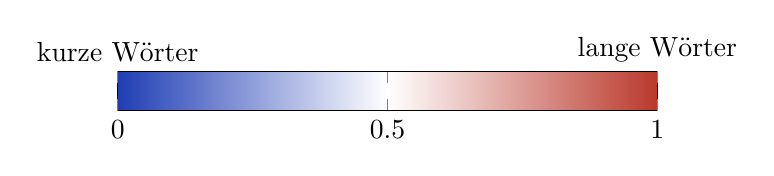
\begin{tikzpicture}
			\begin{axis}[
			colormap={lolmap}{[1cm] 
				rgb255(0cm)=(32,62,181) color(5cm)=(white) rgb255(10cm)=(186,57,44)}, colorbar horizontal, colorbar/width=.5cm, 
				colorbar style={xtick={0,.5,1},
				xlabel near ticks, 
				extra x ticks={0,1},
				extra x tick labels={kurze Wörter, lange Wörter}, 
				extra x tick style={ticklabel pos=right}   
				},
				hide axis
			]
			%\addplot[mesh, point meta=y, line width=4mm, samples=150] {x^2}; % Some graph to show...
			\end{axis}
			\end{tikzpicture}
		\end{figure}
	\subsection*{Komplexität der Vokabeln}
	Hier wird der Prozentanteil eines Absatzes/Satzes gemessen, der nicht in einer Liste häufig verwendeter Wörter vorkommt. Dazu kann entweder Wikipedia\footnote{\url{https://en.wiktionary.org/wiki/Wiktionary:Frequency_lists\#German}} (deutsch/englisch), ein Korpus aus Zeitungsartikeln\footnote{\url{http://wortschatz.uni-leipzig.de/html/wliste.html}} oder evtl. eine fachspezifische Textsammlung ausgewertet werden. Der Anteil der Wörter $ w_i $, die nicht in der Liste $ L $ sind, wird dann durch die Anzahl $ |W| $ der Wörter im zu analysierenden Text $ W $ geteilt, also $  \textit{Komplexität}_W= \frac{|w_i\not\in L|}{|W|}$.\\

		\begin{figure}[h]
			\centering
			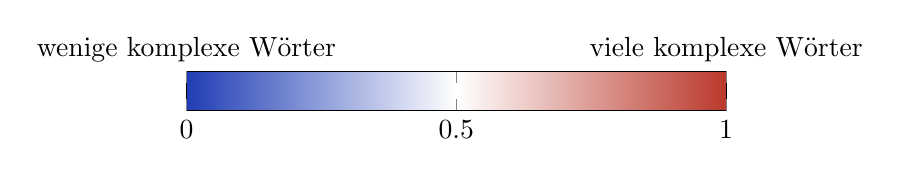
\begin{tikzpicture}
			\begin{axis}[
			colormap={lolmap}{[1cm] 
				rgb255(0cm)=(32,62,181) color(5cm)=(white) rgb255(10cm)=(186,57,44)}, colorbar horizontal, colorbar/width=.5cm, 
			colorbar style={xtick={0,.5,1},
				xlabel near ticks, 
				extra x ticks={0,1},
				extra x tick labels={wenige komplexe Wörter, viele komplexe Wörter}, 
				extra x tick style={ticklabel pos=right}   
			},
			hide axis
			]
			%\addplot[mesh, point meta=y, line width=4mm, samples=150] {x^2}; % Some graph to show...
			\end{axis}
			\end{tikzpicture}
		\end{figure}
		
	\subsection*{Nominalisierungen}
	Die Nominalisierung ist die Bildung eines Substantivs aus einer anderen Wortart, vor allem aus Verben und Adjektiven (z.B. \textit{das Böse, etwas Hübsches; the evil, something pretty}). Ein Gerundium ist ein substantivierter Infinitiv eines Verbs (z.b. \textit{\textbf{climbing} is dangerous; \textbf{das Klettern} ist gefährlich}).
	
	Da Nominalisierungen schwer grundsätzlich vermeidbar sind, die Lesbarkeit des Textes aber auch nicht zwingend schwer unter ihrer Verwendung leidet (z.B. \textit{Es geschah aus \textbf{Versehen}; The \textbf{use} of drugs is dangerous}), muss die Bewertungsskala kontextsensitiv angelegt werden. Bei einem wissenschaftlichen Fachartikel wird die Lesbarkeit bzgl. dieses Kriteriums u.U. zugunsten einer präzisen Formulierung vernachlässigt, in der Unterhaltungsliteratur als Stilmittel, etwa zugunsten einer bestimmten Ausdrucksweise. 
	
	Ein mögliches Maß ist die Anzahl der Nominalisierungen $ |W_{Nominalisierung}| $ geteilt durch die Anzahl der Substantive im zu analysierenden Text $ |W_{Substantive}| $, also $ \textit{Nominalisierungen}_W	=\frac{|W_{Nominalisierung}|}{|W_{Substantive}|} $, wobei $ W_{Nominalisierung}\subseteq W_{Substantive} $. Der resultierende Wert kann wie beim Kriterium Wortlänge normalisiert und farbkodiert werden.\\
	
	\begin{figure}[h]
		\centering
		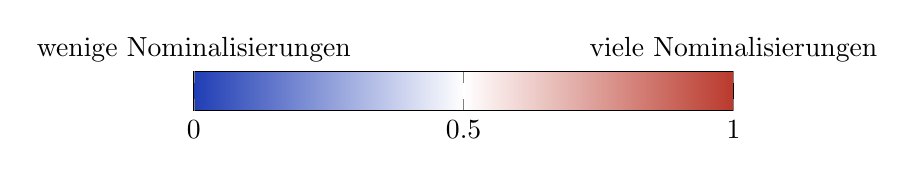
\begin{tikzpicture}
		\begin{axis}[
		colormap={lolmap}{[1cm] 
			rgb255(0cm)=(32,62,181) color(5cm)=(white) rgb255(10cm)=(186,57,44)}, colorbar horizontal, colorbar/width=.5cm, 
		colorbar style={xtick={0,.5,1},
			xlabel near ticks, 
			extra x ticks={0,1},
			extra x tick labels={wenige Nominalisierungen, viele Nominalisierungen}, 
			extra x tick style={ticklabel pos=right}   
		},
		hide axis
		]
		%\addplot[mesh, point meta=y, line width=4mm, samples=150] {x^2}; % Some graph to show...
		\end{axis}
		\end{tikzpicture}
	\end{figure}
	
	\subsection*{Satzlänge}
	Hier wird die Anzahl der Wörter in einem Satz gemessen. Sollte kein Katalog an \textit{Grundwahrheiten} (vgl. Einleitung) gebildet werden, könnten entsprechende Werte aus anderer Literatur\footnote{\url{https://de.wikipedia.org/wiki/Satzlänge\#Durchschnittliche_Satzl.C3.A4nge}} übernommen werden, was jedoch in je nach Kontext (nicht berücksichtige Textarten, Sprachwandel) zu weniger aussagekräftigen Ergebnissen führen könnte.
	
		\begin{figure}[h]
			\centering
			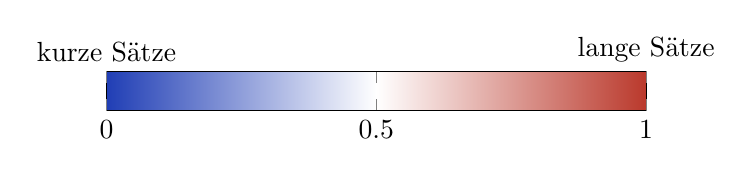
\begin{tikzpicture}
			\begin{axis}[
			colormap={lolmap}{[1cm] 
				rgb255(0cm)=(32,62,181) color(5cm)=(white) rgb255(10cm)=(186,57,44)}, colorbar horizontal, colorbar/width=.5cm, 
			colorbar style={xtick={0,.5,1},
				xlabel near ticks, 
				extra x ticks={0,1},
				extra x tick labels={kurze Sätze, lange Sätze}, 
				extra x tick style={ticklabel pos=right}   
			},
			hide axis
			]
			%\addplot[mesh, point meta=y, line width=4mm, samples=150] {x^2}; % Some graph to show...
			\end{axis}
			\end{tikzpicture}
		\end{figure}
	\subsection*{Komplexität der Satzstruktur}
	Dieses Kriterium basiert auf der Annahme, dass der für das Verständnis eines Satzes erforderliche mentale Arbeitsaufwand mit dem Grad an Verschachtelung und der Verwendung von Klammern steigt. Der Maßstab zugrundeliegende Verzweigungsfaktor des Satzstruktur-Baums muss zunächst experimentell ermittelt werden, etwa mittels NLTK\footnote{\url{http://www.nltk.org/book/ch08.html}}.
	
		\begin{figure}[h]
			\centering
			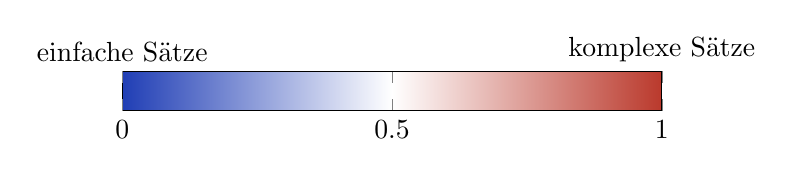
\begin{tikzpicture}
			\begin{axis}[
			colormap={lolmap}{[1cm] 
				rgb255(0cm)=(32,62,181) color(5cm)=(white) rgb255(10cm)=(186,57,44)}, colorbar horizontal, colorbar/width=.5cm, 
			colorbar style={xtick={0,.5,1},
				xlabel near ticks, 
				extra x ticks={0,1},
				extra x tick labels={einfache Sätze, komplexe Sätze}, 
				extra x tick style={ticklabel pos=right}   
			},
			hide axis
			]
			%\addplot[mesh, point meta=y, line width=4mm, samples=150] {x^2}; % Some graph to show...
			\end{axis}
			\end{tikzpicture}
		\end{figure}
\end{document}